% Created by tikzDevice version 0.11 on 2018-04-09 15:27:54
% !TEX encoding = UTF-8 Unicode
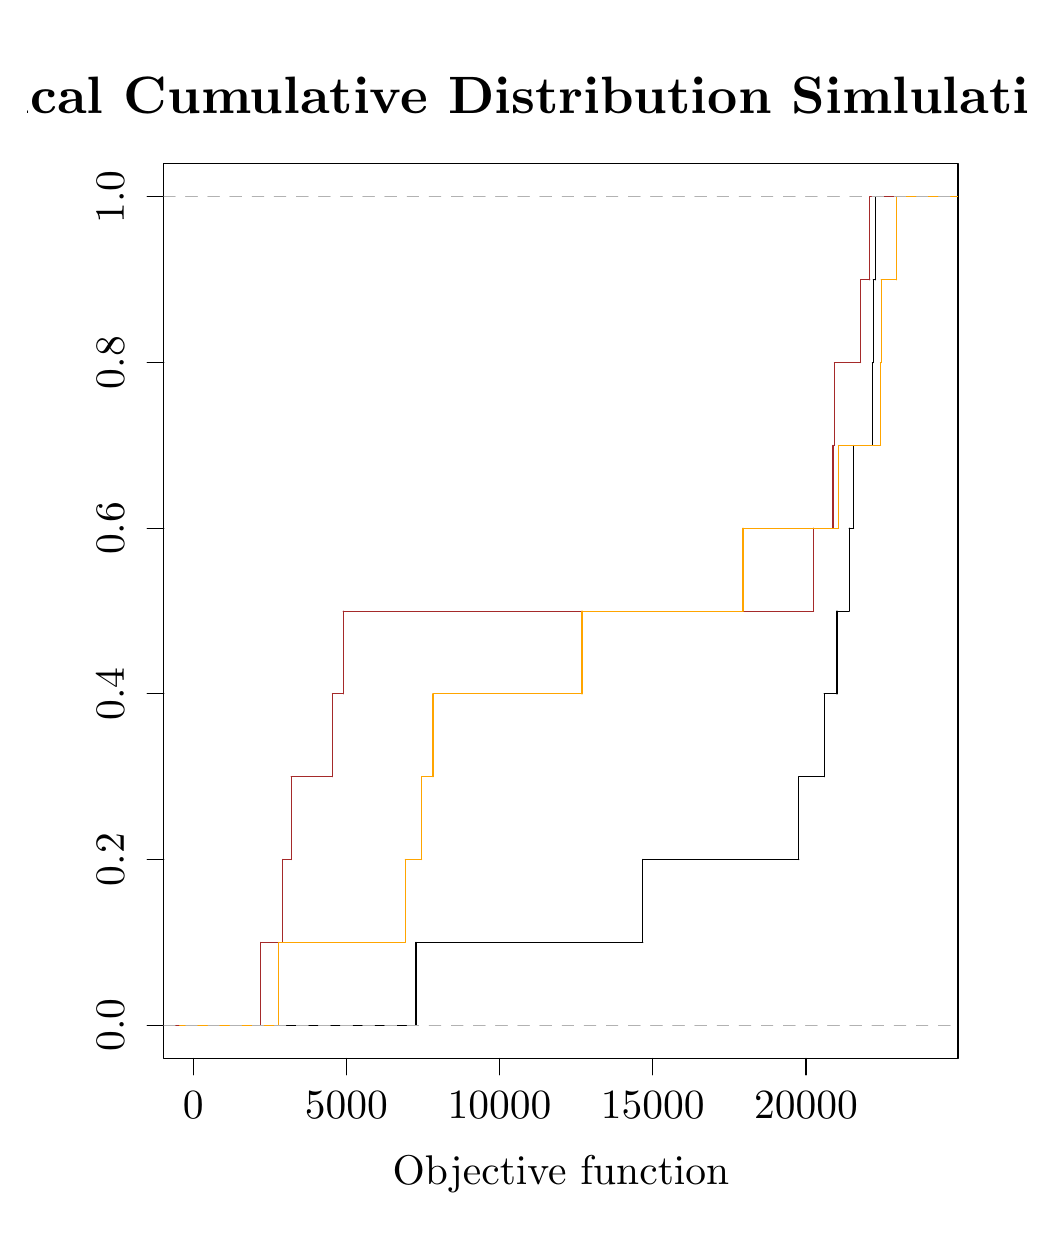
\begin{tikzpicture}[x=1pt,y=1pt]
\definecolor{fillColor}{RGB}{255,255,255}
\path[use as bounding box,fill=fillColor,fill opacity=0.00] (0,0) rectangle (361.35,433.62);
\begin{scope}
\path[clip] (  0.00,  0.00) rectangle (361.35,433.62);
\definecolor{drawColor}{RGB}{0,0,0}

\path[draw=drawColor,line width= 0.4pt,line join=round,line cap=round] ( 59.83, 61.20) -- (281.24, 61.20);

\path[draw=drawColor,line width= 0.4pt,line join=round,line cap=round] ( 59.83, 61.20) -- ( 59.83, 55.20);

\path[draw=drawColor,line width= 0.4pt,line join=round,line cap=round] (115.18, 61.20) -- (115.18, 55.20);

\path[draw=drawColor,line width= 0.4pt,line join=round,line cap=round] (170.53, 61.20) -- (170.53, 55.20);

\path[draw=drawColor,line width= 0.4pt,line join=round,line cap=round] (225.89, 61.20) -- (225.89, 55.20);

\path[draw=drawColor,line width= 0.4pt,line join=round,line cap=round] (281.24, 61.20) -- (281.24, 55.20);

\node[text=drawColor,anchor=base,inner sep=0pt, outer sep=0pt, scale=  1.50] at ( 59.83, 39.60) {0};

\node[text=drawColor,anchor=base,inner sep=0pt, outer sep=0pt, scale=  1.50] at (115.18, 39.60) {5000};

\node[text=drawColor,anchor=base,inner sep=0pt, outer sep=0pt, scale=  1.50] at (170.53, 39.60) {10000};

\node[text=drawColor,anchor=base,inner sep=0pt, outer sep=0pt, scale=  1.50] at (225.89, 39.60) {15000};

\node[text=drawColor,anchor=base,inner sep=0pt, outer sep=0pt, scale=  1.50] at (281.24, 39.60) {20000};

\path[draw=drawColor,line width= 0.4pt,line join=round,line cap=round] ( 49.20, 73.17) -- ( 49.20,372.45);

\path[draw=drawColor,line width= 0.4pt,line join=round,line cap=round] ( 49.20, 73.17) -- ( 43.20, 73.17);

\path[draw=drawColor,line width= 0.4pt,line join=round,line cap=round] ( 49.20,133.03) -- ( 43.20,133.03);

\path[draw=drawColor,line width= 0.4pt,line join=round,line cap=round] ( 49.20,192.88) -- ( 43.20,192.88);

\path[draw=drawColor,line width= 0.4pt,line join=round,line cap=round] ( 49.20,252.74) -- ( 43.20,252.74);

\path[draw=drawColor,line width= 0.4pt,line join=round,line cap=round] ( 49.20,312.59) -- ( 43.20,312.59);

\path[draw=drawColor,line width= 0.4pt,line join=round,line cap=round] ( 49.20,372.45) -- ( 43.20,372.45);

\node[text=drawColor,rotate= 90.00,anchor=base,inner sep=0pt, outer sep=0pt, scale=  1.50] at ( 34.80, 73.17) {0.0};

\node[text=drawColor,rotate= 90.00,anchor=base,inner sep=0pt, outer sep=0pt, scale=  1.50] at ( 34.80,133.03) {0.2};

\node[text=drawColor,rotate= 90.00,anchor=base,inner sep=0pt, outer sep=0pt, scale=  1.50] at ( 34.80,192.88) {0.4};

\node[text=drawColor,rotate= 90.00,anchor=base,inner sep=0pt, outer sep=0pt, scale=  1.50] at ( 34.80,252.74) {0.6};

\node[text=drawColor,rotate= 90.00,anchor=base,inner sep=0pt, outer sep=0pt, scale=  1.50] at ( 34.80,312.59) {0.8};

\node[text=drawColor,rotate= 90.00,anchor=base,inner sep=0pt, outer sep=0pt, scale=  1.50] at ( 34.80,372.45) {1.0};

\path[draw=drawColor,line width= 0.4pt,line join=round,line cap=round] ( 49.20, 61.20) --
	(336.15, 61.20) --
	(336.15,384.42) --
	( 49.20,384.42) --
	( 49.20, 61.20);
\end{scope}
\begin{scope}
\path[clip] (  0.00,  0.00) rectangle (361.35,433.62);
\definecolor{drawColor}{RGB}{0,0,0}

\node[text=drawColor,anchor=base,inner sep=0pt, outer sep=0pt, scale=  1.90] at (192.68,402.46) {\bfseries Empirical Cumulative Distribution Simlulation values};

\node[text=drawColor,anchor=base,inner sep=0pt, outer sep=0pt, scale=  1.50] at (192.68, 15.60) {Objective function};
\end{scope}
\begin{scope}
\path[clip] ( 49.20, 61.20) rectangle (336.15,384.42);
\definecolor{drawColor}{RGB}{0,0,0}

\path[draw=drawColor,line width= 0.4pt,line join=round,line cap=round] (  0.00, 73.17) -- (140.31, 73.17);

\path[draw=drawColor,line width= 0.4pt,line join=round,line cap=round] (140.31,103.10) -- (222.27,103.10);

\path[draw=drawColor,line width= 0.4pt,line join=round,line cap=round] (222.27,133.03) -- (278.66,133.03);

\path[draw=drawColor,line width= 0.4pt,line join=round,line cap=round] (278.66,162.95) -- (287.77,162.95);

\path[draw=drawColor,line width= 0.4pt,line join=round,line cap=round] (287.77,192.88) -- (292.45,192.88);

\path[draw=drawColor,line width= 0.4pt,line join=round,line cap=round] (292.45,222.81) -- (296.85,222.81);

\path[draw=drawColor,line width= 0.4pt,line join=round,line cap=round] (296.85,252.74) -- (298.44,252.74);

\path[draw=drawColor,line width= 0.4pt,line join=round,line cap=round] (298.44,282.67) -- (305.21,282.67);

\path[draw=drawColor,line width= 0.4pt,line join=round,line cap=round] (305.21,312.59) -- (305.56,312.59);

\path[draw=drawColor,line width= 0.4pt,line join=round,line cap=round] (305.56,342.52) -- (306.29,342.52);

\path[draw=drawColor,line width= 0.4pt,line join=round,line cap=round] (306.29,372.45) -- (361.35,372.45);

\path[draw=drawColor,line width= 0.4pt,line join=round,line cap=round] (140.31, 73.17) -- (140.31,103.10);

\path[draw=drawColor,line width= 0.4pt,line join=round,line cap=round] (222.27,103.10) -- (222.27,133.03);

\path[draw=drawColor,line width= 0.4pt,line join=round,line cap=round] (278.66,133.03) -- (278.66,162.95);

\path[draw=drawColor,line width= 0.4pt,line join=round,line cap=round] (287.77,162.95) -- (287.77,192.88);

\path[draw=drawColor,line width= 0.4pt,line join=round,line cap=round] (292.45,192.88) -- (292.45,222.81);

\path[draw=drawColor,line width= 0.4pt,line join=round,line cap=round] (296.85,222.81) -- (296.85,252.74);

\path[draw=drawColor,line width= 0.4pt,line join=round,line cap=round] (298.44,252.74) -- (298.44,282.67);

\path[draw=drawColor,line width= 0.4pt,line join=round,line cap=round] (305.21,282.67) -- (305.21,312.59);

\path[draw=drawColor,line width= 0.4pt,line join=round,line cap=round] (305.56,312.59) -- (305.56,342.52);

\path[draw=drawColor,line width= 0.4pt,line join=round,line cap=round] (306.29,342.52) -- (306.29,372.45);
\definecolor{drawColor}{gray}{0.70}

\path[draw=drawColor,line width= 0.4pt,dash pattern=on 4pt off 4pt ,line join=round,line cap=round] ( 49.20, 73.17) -- (336.15, 73.17);

\path[draw=drawColor,line width= 0.4pt,dash pattern=on 4pt off 4pt ,line join=round,line cap=round] ( 49.20,372.45) -- (336.15,372.45);
\definecolor{drawColor}{RGB}{165,42,42}

\path[draw=drawColor,line width= 0.4pt,line join=round,line cap=round] ( 49.02, 73.17) -- ( 84.23, 73.17);

\path[draw=drawColor,line width= 0.4pt,line join=round,line cap=round] ( 84.23,103.10) -- ( 92.11,103.10);

\path[draw=drawColor,line width= 0.4pt,line join=round,line cap=round] ( 92.11,133.03) -- ( 95.23,133.03);

\path[draw=drawColor,line width= 0.4pt,line join=round,line cap=round] ( 95.23,162.95) -- (110.09,162.95);

\path[draw=drawColor,line width= 0.4pt,line join=round,line cap=round] (110.09,192.88) -- (114.02,192.88);

\path[draw=drawColor,line width= 0.4pt,line join=round,line cap=round] (114.02,222.81) -- (283.95,222.81);

\path[draw=drawColor,line width= 0.4pt,line join=round,line cap=round] (283.95,252.74) -- (290.99,252.74);

\path[draw=drawColor,line width= 0.4pt,line join=round,line cap=round] (290.99,282.67) -- (291.55,282.67);

\path[draw=drawColor,line width= 0.4pt,line join=round,line cap=round] (291.55,312.59) -- (300.99,312.59);

\path[draw=drawColor,line width= 0.4pt,line join=round,line cap=round] (300.99,342.52) -- (304.27,342.52);

\path[draw=drawColor,line width= 0.4pt,line join=round,line cap=round] (304.27,372.45) -- (339.47,372.45);

\path[draw=drawColor,line width= 0.4pt,line join=round,line cap=round] ( 84.23, 73.17) -- ( 84.23,103.10);

\path[draw=drawColor,line width= 0.4pt,line join=round,line cap=round] ( 92.11,103.10) -- ( 92.11,133.03);

\path[draw=drawColor,line width= 0.4pt,line join=round,line cap=round] ( 95.23,133.03) -- ( 95.23,162.95);

\path[draw=drawColor,line width= 0.4pt,line join=round,line cap=round] (110.09,162.95) -- (110.09,192.88);

\path[draw=drawColor,line width= 0.4pt,line join=round,line cap=round] (114.02,192.88) -- (114.02,222.81);

\path[draw=drawColor,line width= 0.4pt,line join=round,line cap=round] (283.95,222.81) -- (283.95,252.74);

\path[draw=drawColor,line width= 0.4pt,line join=round,line cap=round] (290.99,252.74) -- (290.99,282.67);

\path[draw=drawColor,line width= 0.4pt,line join=round,line cap=round] (291.55,282.67) -- (291.55,312.59);

\path[draw=drawColor,line width= 0.4pt,line join=round,line cap=round] (300.99,312.59) -- (300.99,342.52);

\path[draw=drawColor,line width= 0.4pt,line join=round,line cap=round] (304.27,342.52) -- (304.27,372.45);
\definecolor{drawColor}{gray}{0.70}

\path[draw=drawColor,line width= 0.4pt,dash pattern=on 4pt off 4pt ,line join=round,line cap=round] ( 49.20, 73.17) -- (336.15, 73.17);

\path[draw=drawColor,line width= 0.4pt,dash pattern=on 4pt off 4pt ,line join=round,line cap=round] ( 49.20,372.45) -- (336.15,372.45);
\definecolor{drawColor}{RGB}{255,165,0}

\path[draw=drawColor,line width= 0.4pt,line join=round,line cap=round] ( 54.93, 73.17) -- ( 90.66, 73.17);

\path[draw=drawColor,line width= 0.4pt,line join=round,line cap=round] ( 90.66,103.10) -- (136.45,103.10);

\path[draw=drawColor,line width= 0.4pt,line join=round,line cap=round] (136.45,133.03) -- (142.33,133.03);

\path[draw=drawColor,line width= 0.4pt,line join=round,line cap=round] (142.33,162.95) -- (146.47,162.95);

\path[draw=drawColor,line width= 0.4pt,line join=round,line cap=round] (146.47,192.88) -- (200.32,192.88);

\path[draw=drawColor,line width= 0.4pt,line join=round,line cap=round] (200.32,222.81) -- (258.47,222.81);

\path[draw=drawColor,line width= 0.4pt,line join=round,line cap=round] (258.47,252.74) -- (293.00,252.74);

\path[draw=drawColor,line width= 0.4pt,line join=round,line cap=round] (293.00,282.67) -- (308.15,282.67);

\path[draw=drawColor,line width= 0.4pt,line join=round,line cap=round] (308.15,312.59) -- (308.42,312.59);

\path[draw=drawColor,line width= 0.4pt,line join=round,line cap=round] (308.42,342.52) -- (314.00,342.52);

\path[draw=drawColor,line width= 0.4pt,line join=round,line cap=round] (314.00,372.45) -- (349.73,372.45);

\path[draw=drawColor,line width= 0.4pt,line join=round,line cap=round] ( 90.66, 73.17) -- ( 90.66,103.10);

\path[draw=drawColor,line width= 0.4pt,line join=round,line cap=round] (136.45,103.10) -- (136.45,133.03);

\path[draw=drawColor,line width= 0.4pt,line join=round,line cap=round] (142.33,133.03) -- (142.33,162.95);

\path[draw=drawColor,line width= 0.4pt,line join=round,line cap=round] (146.47,162.95) -- (146.47,192.88);

\path[draw=drawColor,line width= 0.4pt,line join=round,line cap=round] (200.32,192.88) -- (200.32,222.81);

\path[draw=drawColor,line width= 0.4pt,line join=round,line cap=round] (258.47,222.81) -- (258.47,252.74);

\path[draw=drawColor,line width= 0.4pt,line join=round,line cap=round] (293.00,252.74) -- (293.00,282.67);

\path[draw=drawColor,line width= 0.4pt,line join=round,line cap=round] (308.15,282.67) -- (308.15,312.59);

\path[draw=drawColor,line width= 0.4pt,line join=round,line cap=round] (308.42,312.59) -- (308.42,342.52);

\path[draw=drawColor,line width= 0.4pt,line join=round,line cap=round] (314.00,342.52) -- (314.00,372.45);
\definecolor{drawColor}{gray}{0.70}

\path[draw=drawColor,line width= 0.4pt,dash pattern=on 4pt off 4pt ,line join=round,line cap=round] ( 49.20, 73.17) -- (336.15, 73.17);

\path[draw=drawColor,line width= 0.4pt,dash pattern=on 4pt off 4pt ,line join=round,line cap=round] ( 49.20,372.45) -- (336.15,372.45);
\end{scope}
\end{tikzpicture}
